\section{Main}
\label{sec:main}
Human “genetic support” implicating genes in disease substantially increases drug target viability and provides a strong justification for experimental studies [Plenge, Minikel, Nelson]. Large-scale genome-wide association studies (GWAS) and exome-wide association studies (ExWAS) provide a strong foundation for this effort. These studies identify hundreds of thousands of variants associated with human traits. However, researchers struggle to determine the specific genes implicated by these associations. Common variant associations often fall in non-coding regions with unclear links to effector genes. Conversely, rare variant associations from ExWAS have limited statistical power. Furthermore, association studies typically report only highly significant associations. These stringent thresholds offer little information on the extent to which sub-significant associations provide genomic support for a gene and trait of interest.

Work to address these challenges mainly falls into three areas. First, effector gene prediction methods attempt to localize significant genome-wide association study (GWAS) signals to specific genes. Fine-mapping methods such as SuSiE[cite] localize GWAS signals to causal variants using sparse priors to calculate better posterior distributions. Fine-mapping is traditionally based on properties of variant association strength but can also be improved by leveraging functional annotations, including ATAC-seq[Corces, Bi], as demonstrated by tools like PolyFun[cite] and fgwas[cite]. These variants can then be linked to putative effector genes using variant-to-gene (V2G) scores that integrate multiple types of evidence (e.g. Hi-C[Jung], cS2G[Gazal]). These predictions are often manually combined into “effector gene lists” that accompany GWAS papers, although these lists lack standardization and rigor[Costanzo]. Second, gene-level approaches such as MAGMA[cite] and MetaXcan[cite] assign genetic support statistics to all genes in the genome by integrating multiple SNPs with (potentially) eQTLs. Third, data from ExWAS, in which burden[cite] or variance component tests[cite] aggregate heuristic masks[Trang] of variants can directly implicate disease-relevant genes, albeit with significantly less power than GWAS[19, Dornbos]. These data and methods each address various parts of the genetic support question, but their heterogeneous assumptions and mathematical frameworks make their integration difficult[HuGE].

To navigate this complexity, we developed a Bayesian statistical method named FALCON (Framework for Analysis of Linkage and Combined Omics using Networks). This model integrates association studies—taking into account correlation— with functional genomic datasets (functional annotations and V2G) to calculate genetic support. We built the network's architecture upon established genetic algorithms (e.g. SuSiE[cite]) and used empirically generated data as priors to inform this structure (e.g. LD Score regression[cite]). We validated the accuracy of this framework on both simulations and real data, using these results to identify the genetic and genomic features most useful for predicting genetic support. We applied FALCON to 1370 full GWAS summary statistics with a total of 117,748 curated GWAS lead SNPs to produce a Genetic Map (G-Map). We used this map to (a) conduct a retrospective analysis of drug target relative success; (b) uncover distinct tissue-mediated mechanisms between SNPs and genes; (c) and evaluate the utility of GWAS associations for prioritizing rare disease genes. This method and map provides a foundation to accurately estimate probabilities of genetic support between every gene and every complex trait.
\section{Results}
\label{sec:results}
\section{Overview of FALCON}
\label{sec:overview}
FALCON is a probabilistic framework designed to model rare and common genetic associations and auxiliary epigenomic annotations as a function of an unknown variable quantifying a gene’s genetic support. FALCON directly ingests standard association statistics while accounting for linkage disequilibrium and environmental noise, seamlessly integrating both common and rare variants by tailoring their underlying hyperparameter distributions. To inform its predictive priors, the model synthesizes diverse functional genomic annotations—including accessible chromatin, enhancers, and loss-of-function metrics—alongside sophisticated variant-to-gene (V2G) linkage scores derived from 3D DNA looping and eQTL mapping (see Supplemental Material). By anchoring on specific genes and evaluating them against all available genomic data and competing targets, FALCON introduces a “reverse genetics” approach that provides a foundation for identifying true causal associations.

In brief, FALCON models observed genetic association data, genomic annotations and linkage scores as a function of a primary latent variable for a gene’s probability of disease relevance and secondary latent variables for variant probability, annotation relevance and linkage probability.

[Equation that shows the rigor used in FALCON here]

The primary output of this framework is gene genetic support—the posterior probability that a specific gene is functionally associated with a trait, conditioned on all observed data. This score—calculated via Gibbs sampling— serves as a standardized metric to evaluate genes within a high-dimensional phenotype space. Furthermore, FALCON’s architecture simultaneously yields secondary outputs, including variant causal probability, fine-mapping, and fine-linking to identify the most likely target genes. Together, these probabilistic outputs generate an end-to-end map translating genetic variation into actionable insight to undercover functional biology (Fig. 1c).

We validated FALCON’s architecture using simulations across diverse trait architectures and sample sizes. Based on Normalized Discounted Cumulative Gain (NDCG)[cite], FALCON’s capacity to recover true disease-relevant genes was nearly optimal, reaching saturation at sample sizes where standard gene-level approaches continued to struggle. Implementation of the model in different scenarios demonstrated shows the importance of combined data. Removal of functional annotations caused a ~60% performance drop in smaller cohorts, while the simultaneous removal of both annotations and linkages reduced an extra ~30% in large-scale datasets (Fig. 1d).

Finally, we confirmed FALCON’s performance on real-world data by evaluating ten UK Biobank traits—representing a broad heritability spectrum 10–55%— utilizing exome-derived rare-variant burden tests as an independent ground truth. Using adapted Gini[cite] and NDCG metrics to assess ranking inequality and prioritization, FALCON demonstrated an ability to separate true biological signals from noise, rapidly concentrating highly relevant genes at the top of its rankings (Fig. 1e, 1f).
\begin{figure}[h!]
    \centering
    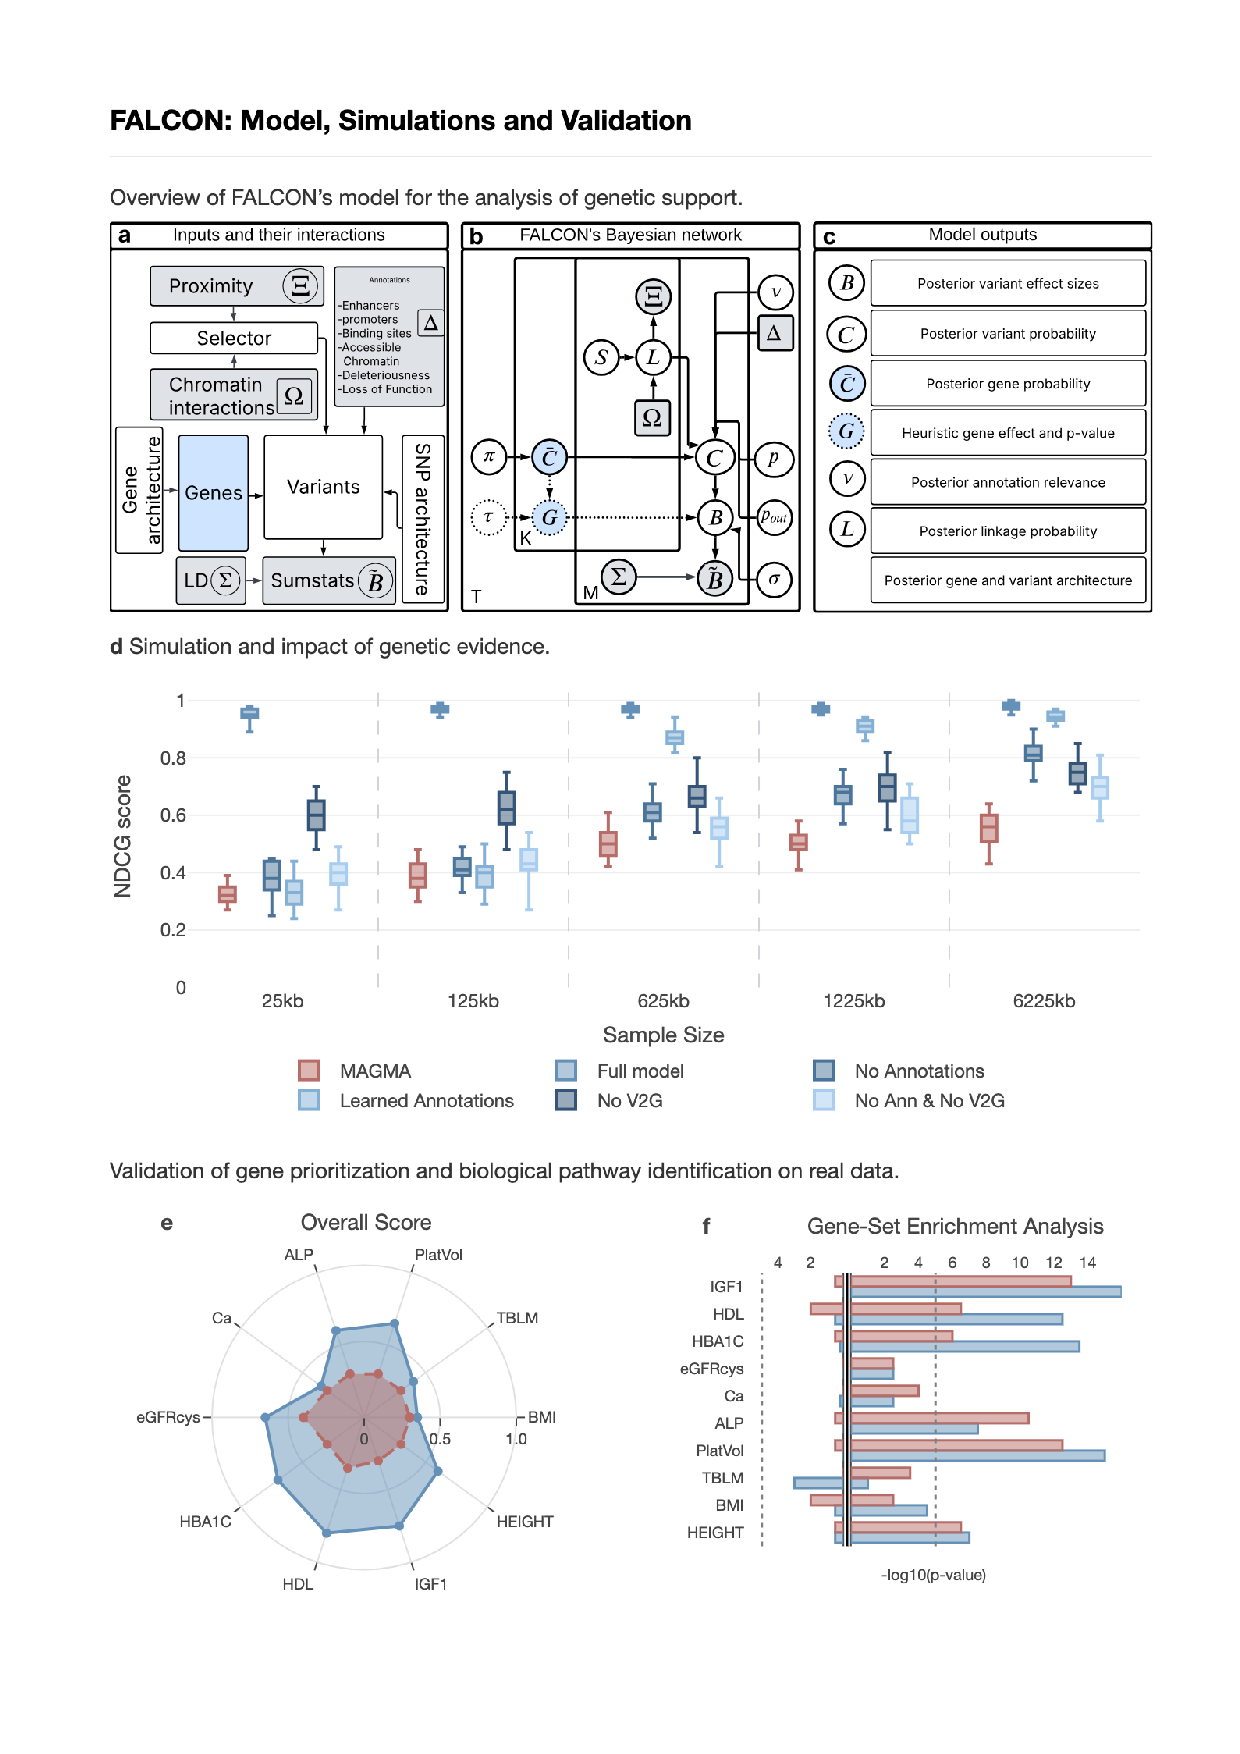
\includegraphics[width=\textwidth]{figures/fig_1.pdf}
\end{figure}

\paragraph{Figure 1.}
a, outlines the diverse data types integrated by the model. The primary inputs include summary statistics (can be GWAS or ExWAS), linkage disequilibrium patterns, functional annotations such as enhancer, promoters, binding sites and accessible chromatin locations for GWAS or deleteriousness and loss of function for ExWAS, and chromatin interaction scores that link regulatory regions to genes. These data sources provide the evidence used to infer association. b, FALCON's core is represented as a Bayesian network, a graphical model that illustrates the probabilistic dependencies between variables. Observed variables (shaded) represent the input data from panel (a). Latent variables (unshaded) represent the unobserved quantities the model aims to estimate. Inference within this network involves two types of information flow: Predictive propagation where information flows from a parent node to a child. For example, functional annotations inform on the probability that a variant is causal. And retrospective propagation a bottom-up flow where observed data at a child node updates beliefs about its parent. For example, the observed summary statistics are used to infer the variant's effect size. c, lists the primary outputs generated by FALCON, which are the posterior probabilities of the latent variables. These posteriors quantify the model's confidence in its inferences, such as the probability that a specific variant is the causal driver of an association signal (posterior variant probability) or that a particular gene is associated to a trait (posterior gene probability). d The figure compares the performance of FALCON (blue) and MAGMA (red) in identifying causal genes across simulated datasets. The performance is measured by the NDCG score (y-axis) at different sample sizes (x-axis, representing thousands of individuals). a, Full model: When FALCON is provided with the correct ("true") functional annotations, it dramatically outperforms MAGMA across all sample sizes. b, No Annotations: annotations are removed and V2G + Weibull is kept. In this scenario FALCON's performance decreases significantly. This highlights the critical role annotations play in improving accuracy. c, Learned Annotations: This panel shows FALCON's ability to learn annotation relevance from data. While not as powerful as using true annotations, this feature allows FALCON to partially recover its performance and still maintain a clear advantage over MAGMA, especially at larger sample sizes. d, No V2G: annotations are kept and V2G + Weibull is removed. Compared to the Full model, the performance (NDCG score) dropped by ~35% at a sample size of 25k and by ~23% at a sample size of 6.2M. e, No Annotations - No V2G: both annotations and V2G + Weibull are removed from FALCON. This setup allows us to evaluate both models under identical data and conditions. Across all tested sample sizes, FALCON consistently outperforms MAGMA. Notably, this performance gap widens with larger sample sizes, indicating that FALCON is more effective at leveraging increased statistical power to accurately identify disease-relevant genes. e, a radar plot visualizing the overall performance score, calculated by averaging the normalized Gini and DCG metrics, across 10 diverse traits. FALCON consistently and substantially outperforms MAGMA across all tested traits. f, gene-set enrichment analysis for positive and negative control pathways across multiple traits. FALCON consistently identifies known, trait-relevant pathways (Positive Control) with much higher statistical significance than MAGMA.

\section{Contribution of different data types to genetic support}
\label{sec:data_types}
The integrated model of FALCON offered the opportunity to quantify which genetic and genomic datasets are most valuable for calculating genetic support. We used simulated data [...]. We [addressed three questions]

Simulated data: What matters What is most valuable to collect

Real data: GWAS vs exomes Empirical statistics (focus on change – does gene prioritization depends on V2G, how much, results on cause analysis both) Show that there are cases of variant to gene changing, but downstream impact on aggregated gene scores is less

Use results of real world ablation to estimate how much S2G or epigenomics we’re missing today. By comparing the difference between the accuracy change in simulation (complete and 100% accurate V2G) vs real data. What change are we going to measure? Real data does not have accuracy. We can calculate the difference in the total number of strong associations.

Sensitivity to parameters, using learned hyperparameters (e.g. LD-score 4th moments and S-LDSC). Difference between a fixed parameter from data. Or calculated by falcon, what prior do we use when learning, same but just let falcon update. A better option would be a random prior, with some set to the learned by data.

Using simulated datasets, these scenarios demonstrate the contribution of functional annotations and linkage data. While the relevance of individual annotations is often unknown a priori, techniques such as partitioned LDSC regression can provide initial estimates that FALCON incorporates to improve precision. However, when external priors are unavailable, FALCON dynamically learns annotation relevance directly from the data. By recovering these functional weights, FALCON maintains precision and outperforms existing baseline models (Fig. 1d).
\section{The HUGEST- Map}
\label{sec:map}
To provide a catalog of human genetic support, we constructed the Genetic Map (G-Map) by applying FALCON on 1,370 bottom-line traits from the Knowledge Portal[cite] across 19,427 genes. The map establishes 208,854 Strong trait-gene associations, defined by a probability threshold of 0.34 based on the Jeffreys Scale with a 5.0% prior[cite].

On average, individual traits are Strong associated with 152 genes. Conversely, 16,333 genes possess at least one Strong trait association, with 1,848 of these genes being associated with exactly one.

The network encompasses 118,177 distinct loci. The map identifies the nearest gene as the top candidate (the gene with the highest probability in the locus) on 73.38% of loci; replicating other studies ([stacy], [Mountjoy]). When examining gene associations for each locus, the majority 52.24% are associated with a single gene (Fig. 3d).

Using relative success rate[cite], we calculated that genes with Strong genetic support from the G-Map are 3.50 times more likely to possess a functional drug target. Compared to the 2.70 rate from the baseline nearest-gene approach, this represents a 29.63% improvement.

Using the curated list of effector genes in [Constanzo] and clinical information from open targets, The G-Map identified 203,214 novel gene-trait associations with and average of 148 novel genes per trait. From the subset of associations with no clinical trials, 16,380 have approved drug targets for the associated gene, making them prime candidates for rapid clinical repurposing.

By integrating the curated list of effector genes from [Constanzo] with clinical data from Open Targets, we systematically categorized the G-Map associations to funnel associations from established therapeutics down to novel discoveries. Within the clinical space, the network captures 1,555 established gene-trait associations. Expanding beyond active clinical trials into translational opportunities, we identified 16,380 associations involving genes with approved drug targets for other indications, rendering them prime candidates for rapid clinical repurposing. Finally, filtering the network for strictly uncharacterized targets uncovers an expansive frontier of 203,214 novel gene-trait associations, driven by an average of 148 novel genes per trait.
\section{Coverage}
\label{sec:coverage}
To evaluate trait representation in the G-Map across established phenotypes, we performed a coverage analysis using the Mondo Disease Ontology [cite]. We employed PubMedBERT to calculate semantic similarity, mapping G-Map trait names directly to ontology terms. Applying a similarity threshold of 0.5 at level 3 of the ontology yielded a match success rate of 94.59% and an overall trait coverage of 57.58%. Within this setup, each trait mapped to an average of 2.3 ontology terms, resulting in a total of 2,972 mappings on 1294 unique traits. Furthermore, the semantic similarity scores for these matched traits had a median of 0.74 (IQR, 0.66–0.84).

Analysis of the matched terms revealed distinct patterns in trait representation across the ontology. The categories exhibiting the highest proportional coverage were acute stress disorder and perinatal disease (both at 50%). In terms of absolute frequency, the most heavily represented categories within the G-Map included diseases of genetic or genomic mechanisms (609), nervous system disorders (296), and metabolic diseases (215).
\section{Overview of genetic architecture}
\label{sec:gen_arch}
To accurately capture the underlying genetic architecture and mitigate the redundancy and low power in GWAS cohorts, it is necessary to evaluate these associations through a bias-adjusted framework. Raw association counts often inflate genetic signals; thus, correcting for this bias is essential to represent a more accurate biological distribution of pleiotropy and polygenicity. By filtering out noise, this bias adjusted analysis shows the biologically active hubs across established clinical therapeutics, repurposable targets and novel discoveries.

The complete, bias corrected G-Map encompasses a network of 16,290 unique genes mapped across 1,152 distinct phenotypic traits, exhibiting a broad pleiotropy (N=7,393) where genes associate with an average of 1.5 traits. The map contains pleiotropic master regulators, with the most dominant genetic signals emerging from PBX2, NOTCH4, and TSBP1 (the three of them with ~40 Strong associated traits). Phenotypically, global genetic burden is driven by undetermined stroke etiology (toastUNDETER; 1,872), complex lean mass phenotypes (TB-LM; 1,815), and platelet volume (PlatVol; 1,692). Consequently, the broadest categorical signals across the entire G-Map are deeply concentrated within hematological (17,223), musculoskeletal (4,575), and renal (4,177) domains.

Funneling this global architecture into the clinically validated space, the network captures 490 established therapeutic targets driving 299 distinct clinical phenotypes. The G-Map highlights a strong clinical inclination toward chronic inflammatory and structural conditions, where top genes: TUBB (4.42), TNF (2.78), and NR3C1 (2.69), and traits: ankylosing spondylitis (6.18), chronic obstructive pulmonary disease (COPD; 5.69), and TB-LM (4.84), modulate microtubule dynamics, systemic inflammation, and glucocorticoid signaling. Expanding beyond established indications, the repurposable class identifies [total|Genes\_Repurposable] genes and [total|Traits\_Repurposable] traits, providing a baseline for immediate translational opportunities. In this repurposable context, the strongest gene candidates are heavily anchored in immune regulation and the major histocompatibility complex, led by HLA-DRB1 (36.01), AGER (32.28), and HLA-DRB5 (30.43). The phenotypic signals and categories driving these repurposable opportunities closely mirror the global baseline.

Finally, filtering the map for novel associations uncovers [total|Genes\_Novel] uncharted biological hubs across [total|Traits\_Novel] distinct traits that have yet to be therapeutically exploited. Within this novel tier, the most dominant genes—PBX2 (40.57), NOTCH4 (40.56), and C6orf10 (40.09)—are identical to the global leaders, emphasizing that the bulk of the network’s untapped pleiotropic potential resides in these developmental and immune-linked loci. The driving traits for these novel discoveries continue to be toastUNDETER (1,872.67), TB-LM (1,810.87), and PlatVol (1,692.64). This alignment firmly establishes the hematological (17,209.32), musculoskeletal (4,467.65), and renal (3,942.39) domains as the primary categories for new target discovery.
\begin{figure}[h!]
    \centering
    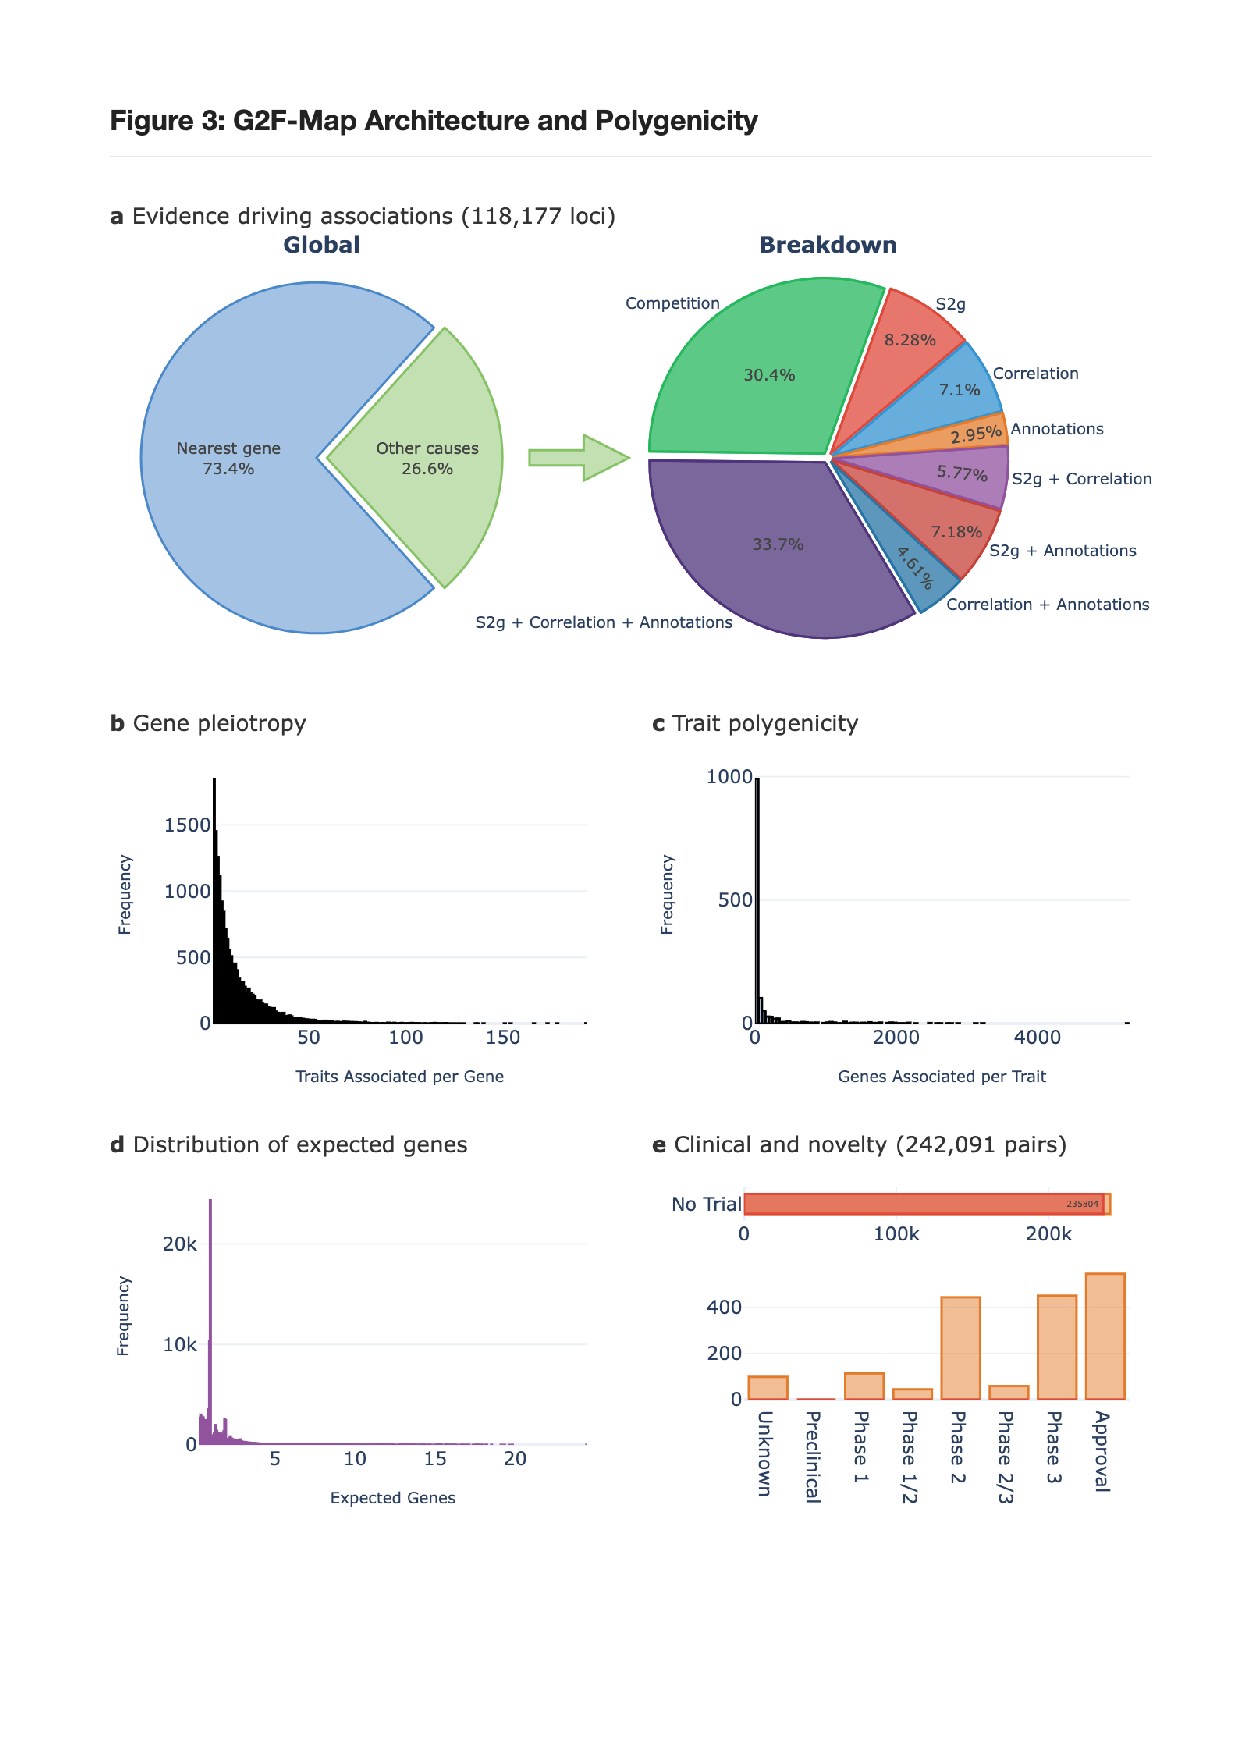
\includegraphics[width=\textwidth]{figures/fig_3.pdf}
\end{figure}

\paragraph{Figure 3.}
a, Shows the distribution of causes …

\begin{figure}[h!]
    \centering
    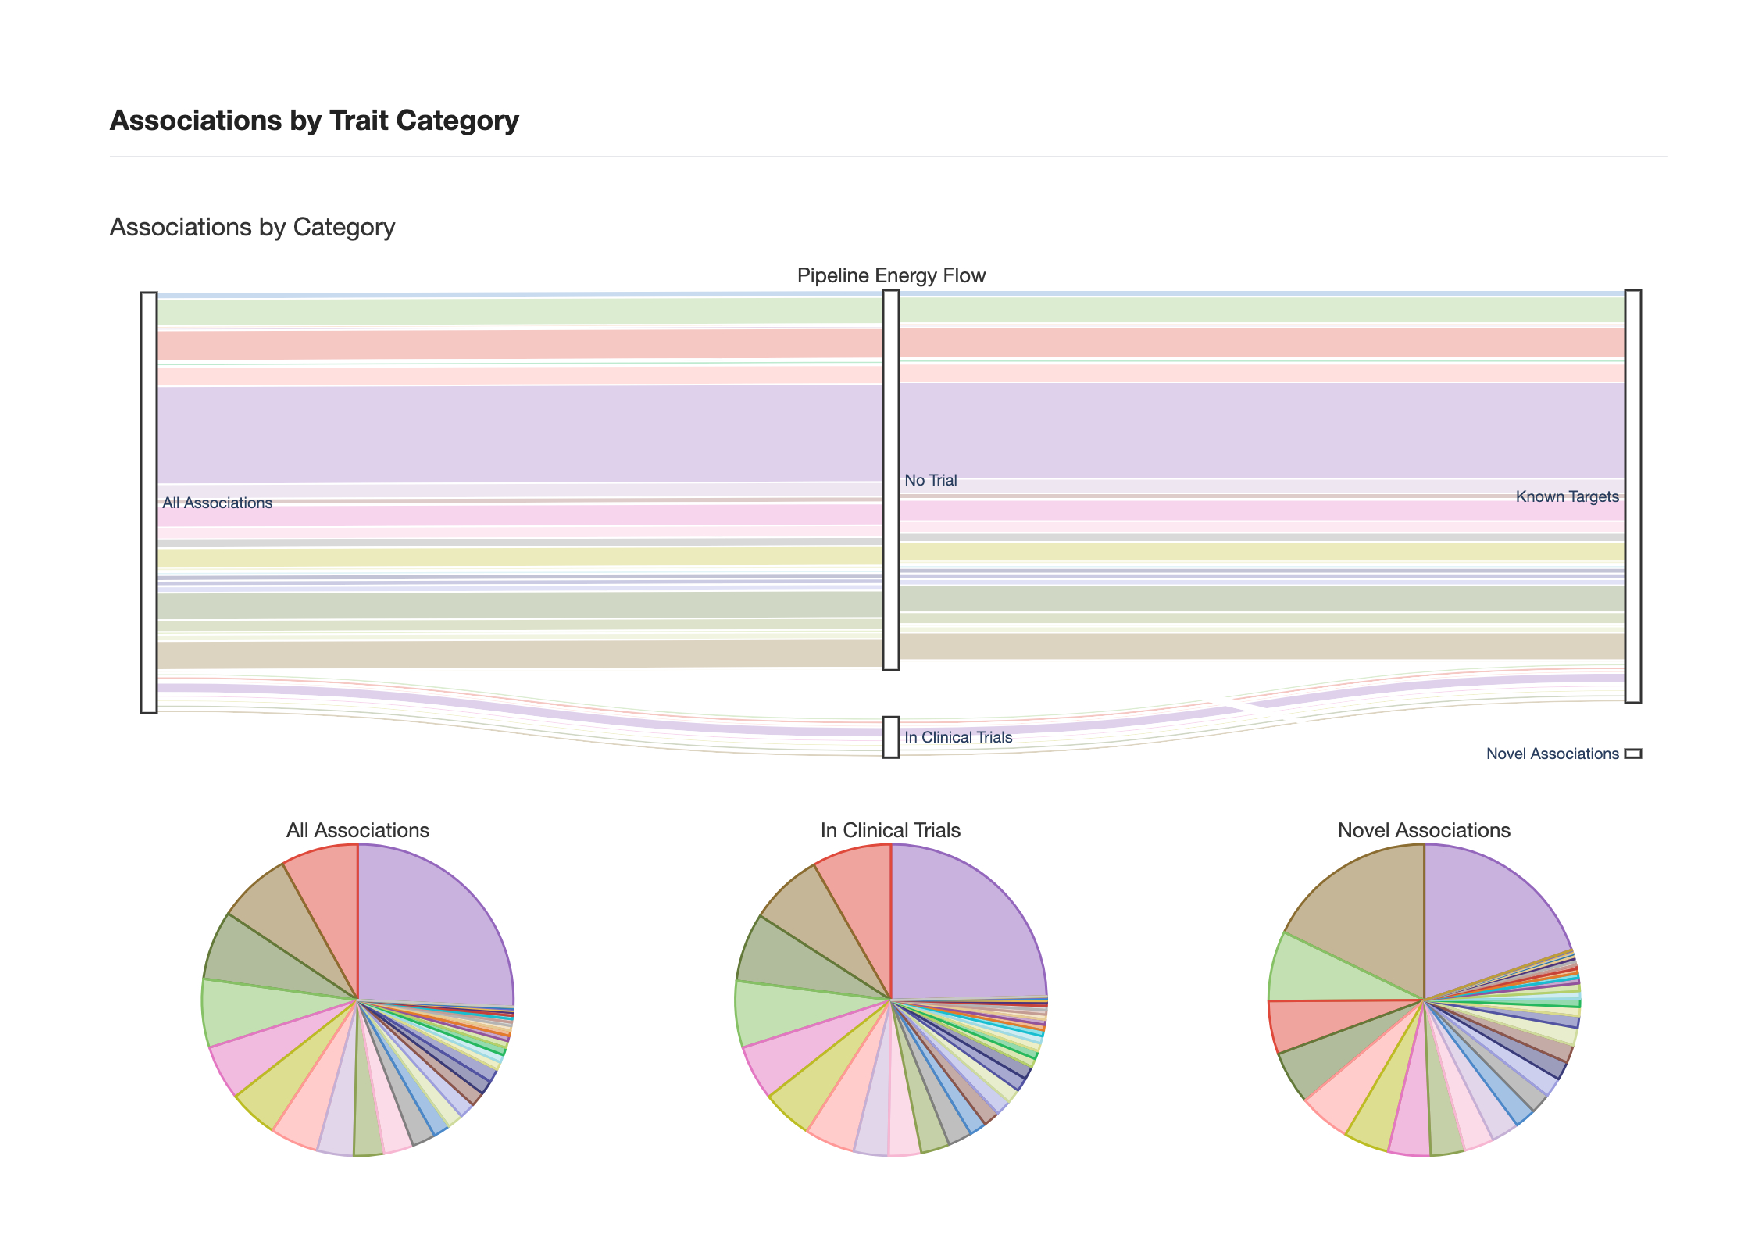
\includegraphics[width=\textwidth]{figures/fig_4.pdf}
\end{figure}

\paragraph{Figure 4.}
a, Shows the distribution of causal genes across categories …

\section{Relative success}
\label{sec:rs}
Drugs target relative success on genes with genetic support. To validate the FALCON resource, we calculated the relative success rate of trait-associated genes as shown in []. We analyzed RS at different thresholds. The analysis (Fig. 4a) showed that genes with FALCON genetic support (at the best threshold) are 3.5 times more likely to have a functional drug target compared to the nearest gene approach (with 2.7). In total there were 900 FALCON genes having a functional drug target, 400 genes that have not been tested for any indication and 500 genes with a functional drug target associated to an indication/trait that has not been tested, these genes having already a functional drug target can be quickly repurposed for the new indication (trait association). It is notable that metabolic traits (e.g. lipid traits or psychiatric traits) are more likely to be repurposable (or lipid traits are XX times more likely to have repurposable genes than psychiatrist traits). This statistical analysis shows how crucial genetic support is needed for better drug target prioritization, showing the model's applicability in accelerating drug discovery.
\section{Leveraging horizontal pleiotropy to improve low powered summary statistics}
\label{sec:horizontal_pleiotropy}
We uncover novel Eosinophilic Esophagitis (EoE) risk loci hidden below standard genome-wide significance thresholds, by integrated sub-significant associations from the Trimarchi 2025 EoE GWAS[cite] with high-powered cross-phenotype data from the G2F-Map. We identified 76 EoE-relevant proxy traits and 30 novel candidate loci. Highlighting the mechanistic utility of this approach, our top targets—CTSB, BCL2L11 (BIM), and RAB27B—map to distinct, sequential stages of the EoE pathogenic cascade, offering genetically validated therapeutic nodes that span initial allergen sensing, prolonged eosinophil survival, and localized mucosal tissue damage.
\section{GWAS vs. ExWAS Comparison}
\label{sec:vs}
Based on the stats after running FALCON. What elements are similar and what is the biggest difference. What are the strengths and weaknesses of each?
\section{Leveraging Insights from Common Diseases to Treat Rare Genetic Disorders}
\label{sec:common_rare}
The vast research dedicated to common diseases can be powerfully repurposed to develop treatments for rare genetic disorders, leveraging the deep molecular understanding gained from studies worth billions of dollars. An example is the use of JAK inhibitors, originally developed to treat common autoimmune diseases like rheumatoid arthritis by dialing down an overactive immune pathway. In a parallel discovery, geneticists found that a rare and devastating immunodeficiency was caused by specific STAT1 gain-of-function mutations that locked this same pathway in a permanently "on" state. This crucial insight allowed for the direct repurposing of existing JAK inhibitors, such as ruxolitinib, to successfully treat these patients, perfectly illustrating how genetic insights from common conditions can provide ready-made cures for rare diseases.
\section{Tissue-mediated mechanisms}
\label{sec:GTT}
When genes exhibit pleiotropy, their effects fall into two distinct structural categories. Tissue-shared pleiotropic (TSP) genes influence related trait families through a single, unified tissue pathway, whereas tissue-distinct pleiotropic (TDP) genes bridge apparently distinct biological domains via completely independent tissues. This gene-side architecture clarifies whether a locus acts narrowly within a specific trait family or coordinates processes across multiple physiological systems.

[Definition 1 / validation 1] As FALCON produced predictions not only of causal genes but also specific variants linked to them and in which tissues those variants are expressed, we asked whether we could classify gene-trait associations into tissue of action. We developed a method to calculate a ToA by summing over variants and blah blah blah. We defined a ToA score to be significant if XXX. Across the XXX pairs, Y (Z%) were significant. Examples include X, Y, and Z (supplementary figure). On average the tissues were more specific than expected by chance, suggesting that most gene trait associations are tissue-specific rather than global. The ToA scores were broadly consistent with gene expression patterns but there were important differences (Figure scatter plot). For example, XXX.

[Definition 2 / validation 2] Of particular interest are genes which are tissue specific for traits as opposed to tissue distinct. We defined TSP-genes vs. TDP-genes as XXX. The definition of TDPs broadly Most (X%) genes were TDP whereas (X%) were TSP (Figure, Supplementary Figure). TDPs were more specific in terms of gene expression patterns than TSPs. Different trait grouping categories were more enriched for TDPs. Correlated traits often share tissues. Constraint? Centrality in PPI networks.

[Why it maps to something real that people reading care about] Drug targetability. Drug Target RS. Side effects. Comparison with exome signals. Core genes.

[Concrete examples] Specific examples of TSP-genes and TDP-genes. Biological insights/consistency.

We have shown how having genetic support helps to understand the biological basis of complex diseases and develop better drug targets. However, it is also essential to determine tissue-specific susceptibilities across different traits on disease-associated genes. Pinpointing the tissues where these genes have their effects can elucidate their functions and identify therapeutic targets. To formalize this concept, we define two categories of pleiotropic genes based on their tissue-mediated mechanisms:

Tissue-Shared Pleiotropic Genes (TSP-genes): These genes influence multiple traits primarily through a single tissue. A canonical example is INS, which affects diabetes-related traits, fasting glucose, and insulin secretion almost exclusively via its activity in the pancreas [cite]. Here, the same tissue mediates diverse phenotypic effects, illustrating unified functional pathways. Tissue-Distinct Pleiotropic Genes (TDP-genes): In contrast, these genes contribute to different traits through independent mechanisms localized at distinct tissues. For instance, HNF1A exhibits two non-colocalized GWAS hits: one linked to type 2 diabetes (T2D) and another to low-density lipoprotein (LDL) levels. The T2D-associated variant likely acts through pancreatic beta-cell dysfunction, while the LDL-linked variant may operate via hepatic lipid metabolism. This tissue-divergent architecture suggests separate causal pathways for each trait, classifying HNF1A as a TDP-gene.

The workflow to find TDPs and TSPs begins by integrating two key data sources: FALCON's results (specifically, the posterior probabilities for variants, genes, and their linkages) and ATAC-seq data, which indicates tissue-specific variant activity. For each gene with sufficient genetic evidence (posterior probability > 0.1) for a set of traits, a "tissue signature" is calculated. This is done by averaging the product of the variant linkage probability and the variant's annotation status for each tissue. The result is a tissue signature matrix, which maps the gene's functional activity across different tissues for multiple traits. Then, we generate the tissue similarity matrix by applying a Jaccard similarity index to the signature matrix. This matrix quantifies the degree of overlap in tissue activity for a single gene across all traits. Finally, genes are classified based on their cross-trait tissue similarity patterns:

TDP genes are identified when the similarity score between two traits falls below a set threshold (e.g., 0.1). This indicates the gene influences each trait through different, or distinct, tissue-specific mechanisms. TSP genes are identified by clustering genes with similar tissue signatures. Genes within the same cluster affect multiple traits through a common, or shared, set of tissues.

After applying this technique to ~1k traits in the KP, We found that X% of the trait-associated genes found by FALCON are Tissue-distinct pleiotropic genes. Providing insight into the degree of tissue-specific regulation and the intricacy of trait architecture (Fig. Xc). We found that HNF1A has at least two tissue-defined mechanisms: primary digestive  on T2D (Stomach, Intestine, Colon) and secondary digestive on LDL (liver, pancreas). In LDL we found that variant rs11065374 has a strong FALCON probability (0.879), cS2G links it to HNF1A (score 1) and overlaps on both secondary digestive tissues. The T2D variant rs6489785 has strong FALCON prob (0.919) and overlaps with 3 of the four primary digestive tissues (Fig. Xd). Results for tissue-specific mechanisms for 4000 traits are all browseable in Portal/resource.





Fig. 6: Tissue-mediated mechanisms.

a, illustrates the workflow for identifying Tissue-Distinct Pleiotropic (TDP) and Tissue-Shared Pleiotropic (TSP) genes. The process integrates FALCON's probabilistic outputs with tissue-specific chromatin accessibility data (ATAC-seq) to uncover how genes influence multiple traits. B, an example of a novel TDP gene, BLID demonstrates tissue-distinct effects, influencing Type 2 Diabetes (left) through the pancreas and liver (orange), and separately affecting High-Density Lipoprotein (right) cholesterol through adipose tissue (blue). Vertical lines show tissue enrichment for the region. c, stats.
\section{Discussion}
\label{sec:discussion}
Data availability Code availability
